% Diagrama de conexiones de la placa ONX3248G035: pantalla, panel táctil,
% microSD y expansor PCF8574.
% Se compila por separado: pdflatex conexiones_onx.tex -> conexiones_onx.pdf
\documentclass[tikz,border=4pt]{standalone}
\usepackage[utf8]{inputenc}
\usepackage[T1]{fontenc}
\usepackage{cmbright}
\usetikzlibrary{arrows.meta}

\definecolor{cspi}{RGB}{31,94,168}
\definecolor{cdir}{RGB}{90,90,90}
\definecolor{csd}{RGB}{30,120,60}
\definecolor{ci2c}{RGB}{190,100,10}
\definecolor{cexp}{RGB}{130,50,140}

\begin{document}
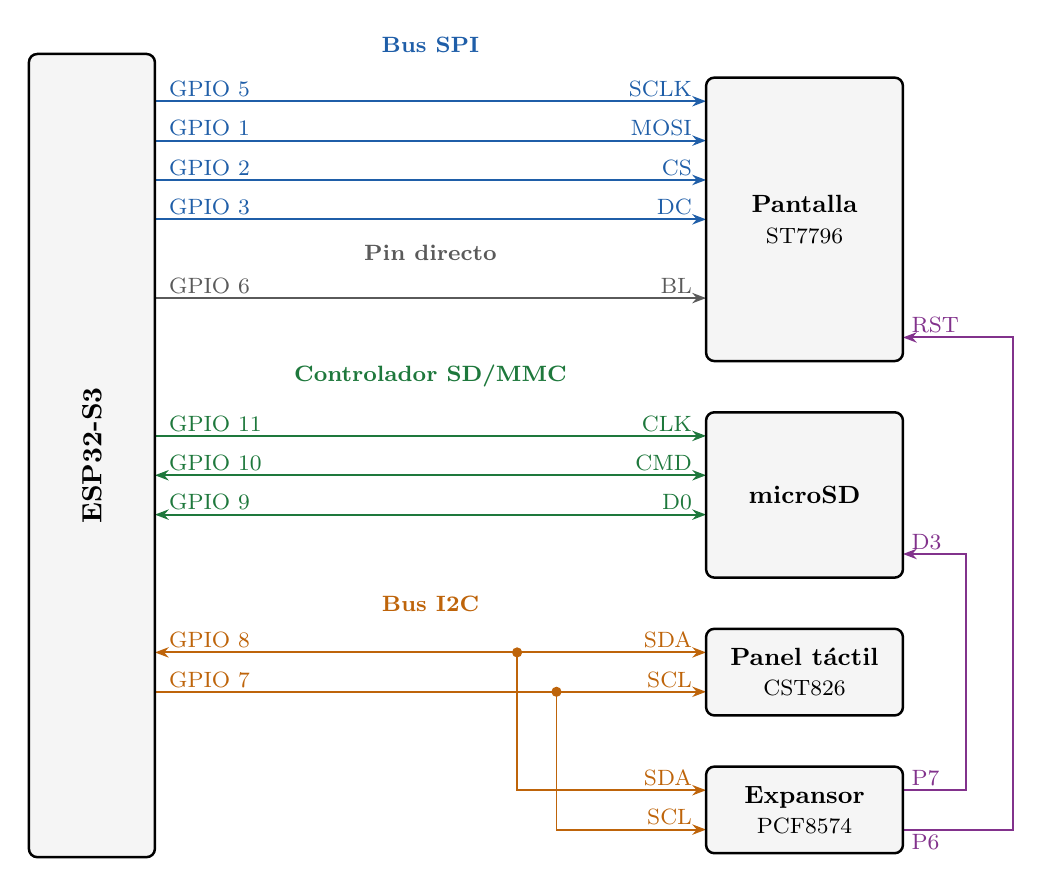
\begin{tikzpicture}[
    font=\small,
    senal/.style={line width=0.7pt},
    caja/.style={draw, line width=0.9pt, rounded corners=3pt, fill=gray!8, align=center},
    gpio/.style={anchor=south west, font=\footnotesize, inner sep=1.5pt},
    nombre/.style={anchor=south east, font=\footnotesize, inner sep=1.5pt},
    grupo/.style={font=\footnotesize\bfseries, anchor=south},
    nodo/.style={circle, fill, inner sep=1.3pt},
    >={Stealth[length=5pt]}
]
\def\xa{0}      % borde derecho del ESP32-S3
\def\xb{7}      % borde izquierdo de los dispositivos
\def\xc{9.5}    % borde derecho de los dispositivos
\def\xg{3.5}    % posición de los rótulos de grupo

% ---------------- Bus SPI: pantalla ----------------
\node[grupo, cspi] at (\xg,0.25) {Bus SPI};
\foreach \n/\g/\y in {SCLK/5/-0.25, MOSI/1/-0.75, CS/2/-1.25, DC/3/-1.75} {
    \draw[senal, cspi, ->] (\xa,\y) -- (\xb,\y);
    \node[gpio, cspi] at (\xa+0.12,\y) {GPIO \g};
    \node[nombre, cspi] at (\xb-0.12,\y) {\n};
}

% ---------------- Pin directo: retroiluminación ----------------
\node[grupo, cdir] at (\xg,-2.4) {Pin directo};
\draw[senal, cdir, ->] (\xa,-2.75) -- (\xb,-2.75);
\node[gpio, cdir] at (\xa+0.12,-2.75) {GPIO 6};
\node[nombre, cdir] at (\xb-0.12,-2.75) {BL};

% ---------------- Controlador SD/MMC: microSD ----------------
\node[grupo, csd] at (\xg,-4.0) {Controlador SD/MMC};
\draw[senal, csd, ->]  (\xa,-4.5) -- (\xb,-4.5);
\draw[senal, csd, <->] (\xa,-5.0) -- (\xb,-5.0);
\draw[senal, csd, <->] (\xa,-5.5) -- (\xb,-5.5);
\foreach \n/\g/\y in {CLK/11/-4.5, CMD/10/-5.0, D0/9/-5.5} {
    \node[gpio, csd] at (\xa+0.12,\y) {GPIO \g};
    \node[nombre, csd] at (\xb-0.12,\y) {\n};
}

% ---------------- Bus I2C: panel táctil y expansor ----------------
\node[grupo, ci2c] at (\xg,-6.85) {Bus I2C};
\draw[senal, ci2c, <->] (\xa,-7.25) -- (\xb,-7.25);
\draw[senal, ci2c, ->]  (\xa,-7.75) -- (\xb,-7.75);
\node[gpio, ci2c] at (\xa+0.12,-7.25) {GPIO 8};
\node[gpio, ci2c] at (\xa+0.12,-7.75) {GPIO 7};
\node[nombre, ci2c] at (\xb-0.12,-7.25) {SDA};
\node[nombre, ci2c] at (\xb-0.12,-7.75) {SCL};
% derivación hacia el expansor
\draw[senal, ci2c, ->] (4.6,-7.25) -- (4.6,-9.0) -- (\xb,-9.0);
\draw[senal, ci2c, ->] (5.1,-7.75) -- (5.1,-9.5) -- (\xb,-9.5);
\node[nodo, ci2c] at (4.6,-7.25) {};
\node[nodo, ci2c] at (5.1,-7.75) {};
\node[nombre, ci2c] at (\xb-0.12,-9.0) {SDA};
\node[nombre, ci2c] at (\xb-0.12,-9.5) {SCL};

% ---------------- Salidas del expansor ----------------
% P7 -> D3 de la microSD; P6 -> RST de la pantalla
\draw[senal, cexp, ->] (\xc,-9.0) -- (10.3,-9.0) -- (10.3,-6.0) -- (\xc,-6.0);
\draw[senal, cexp, ->] (\xc,-9.5) -- (10.9,-9.5) -- (10.9,-3.25) -- (\xc,-3.25);
\node[anchor=south west, font=\footnotesize, inner sep=1.5pt, cexp] at (\xc+0.05,-9.0) {P7};
\node[anchor=north west, font=\footnotesize, inner sep=1.5pt, cexp] at (\xc+0.05,-9.5) {P6};
\node[anchor=south west, font=\footnotesize, inner sep=1.5pt, cexp] at (\xc+0.05,-6.0) {D3};
\node[anchor=south west, font=\footnotesize, inner sep=1.5pt, cexp] at (\xc+0.05,-3.25) {RST};

% ---------------- Bloques ----------------
\draw[caja] (\xa-1.6,0.35) rectangle (\xa,-9.85);
\node[rotate=90, font=\bfseries] at (\xa-0.8,-4.75) {ESP32-S3};

\draw[caja] (\xb,0.05) rectangle (\xc,-3.55);
\node[align=center] at ({(\xb+\xc)/2},-1.75) {\textbf{Pantalla}\\\footnotesize ST7796};

\draw[caja] (\xb,-4.2) rectangle (\xc,-6.3);
\node[align=center] at ({(\xb+\xc)/2},-5.25) {\textbf{microSD}};

\draw[caja] (\xb,-6.95) rectangle (\xc,-8.05);
\node[align=center] at ({(\xb+\xc)/2},-7.5) {\textbf{Panel táctil}\\\footnotesize CST826};

\draw[caja] (\xb,-8.7) rectangle (\xc,-9.8);
\node[align=center] at ({(\xb+\xc)/2},-9.25) {\textbf{Expansor}\\\footnotesize PCF8574};
\end{tikzpicture}
\end{document}
